This section treats the preparation of the petal in the first two subsections and eventually the first results of the thermal performance tests done in late august 2018 in the third subsection.
\subsection{Last Pre-Study on Gluing pt100s and Paint Emissivity on Si}
As outlined in section \ref{sec:emissivity}, the petal needs to be covered with a high emissivity coating. The chosen paint was examined in section \ref{sec:emissivityMeasurement}.
Before the tests could start, we decided to do a last pre-study to check if the paint when sprayed onto Si has the same emissivity as on Aluminium and to check if gluing the pt100s onto Si is as reliable as clamping. The set-up for this test is similar to the one described in \ref{sec:setup}: the same Peltier element sitting in the same cardboard box. The only modifications are on the surface of the Peltier as shown in figure \ref{fig:peltierGlue}.
\begin{figure}[h!]
	\centering
	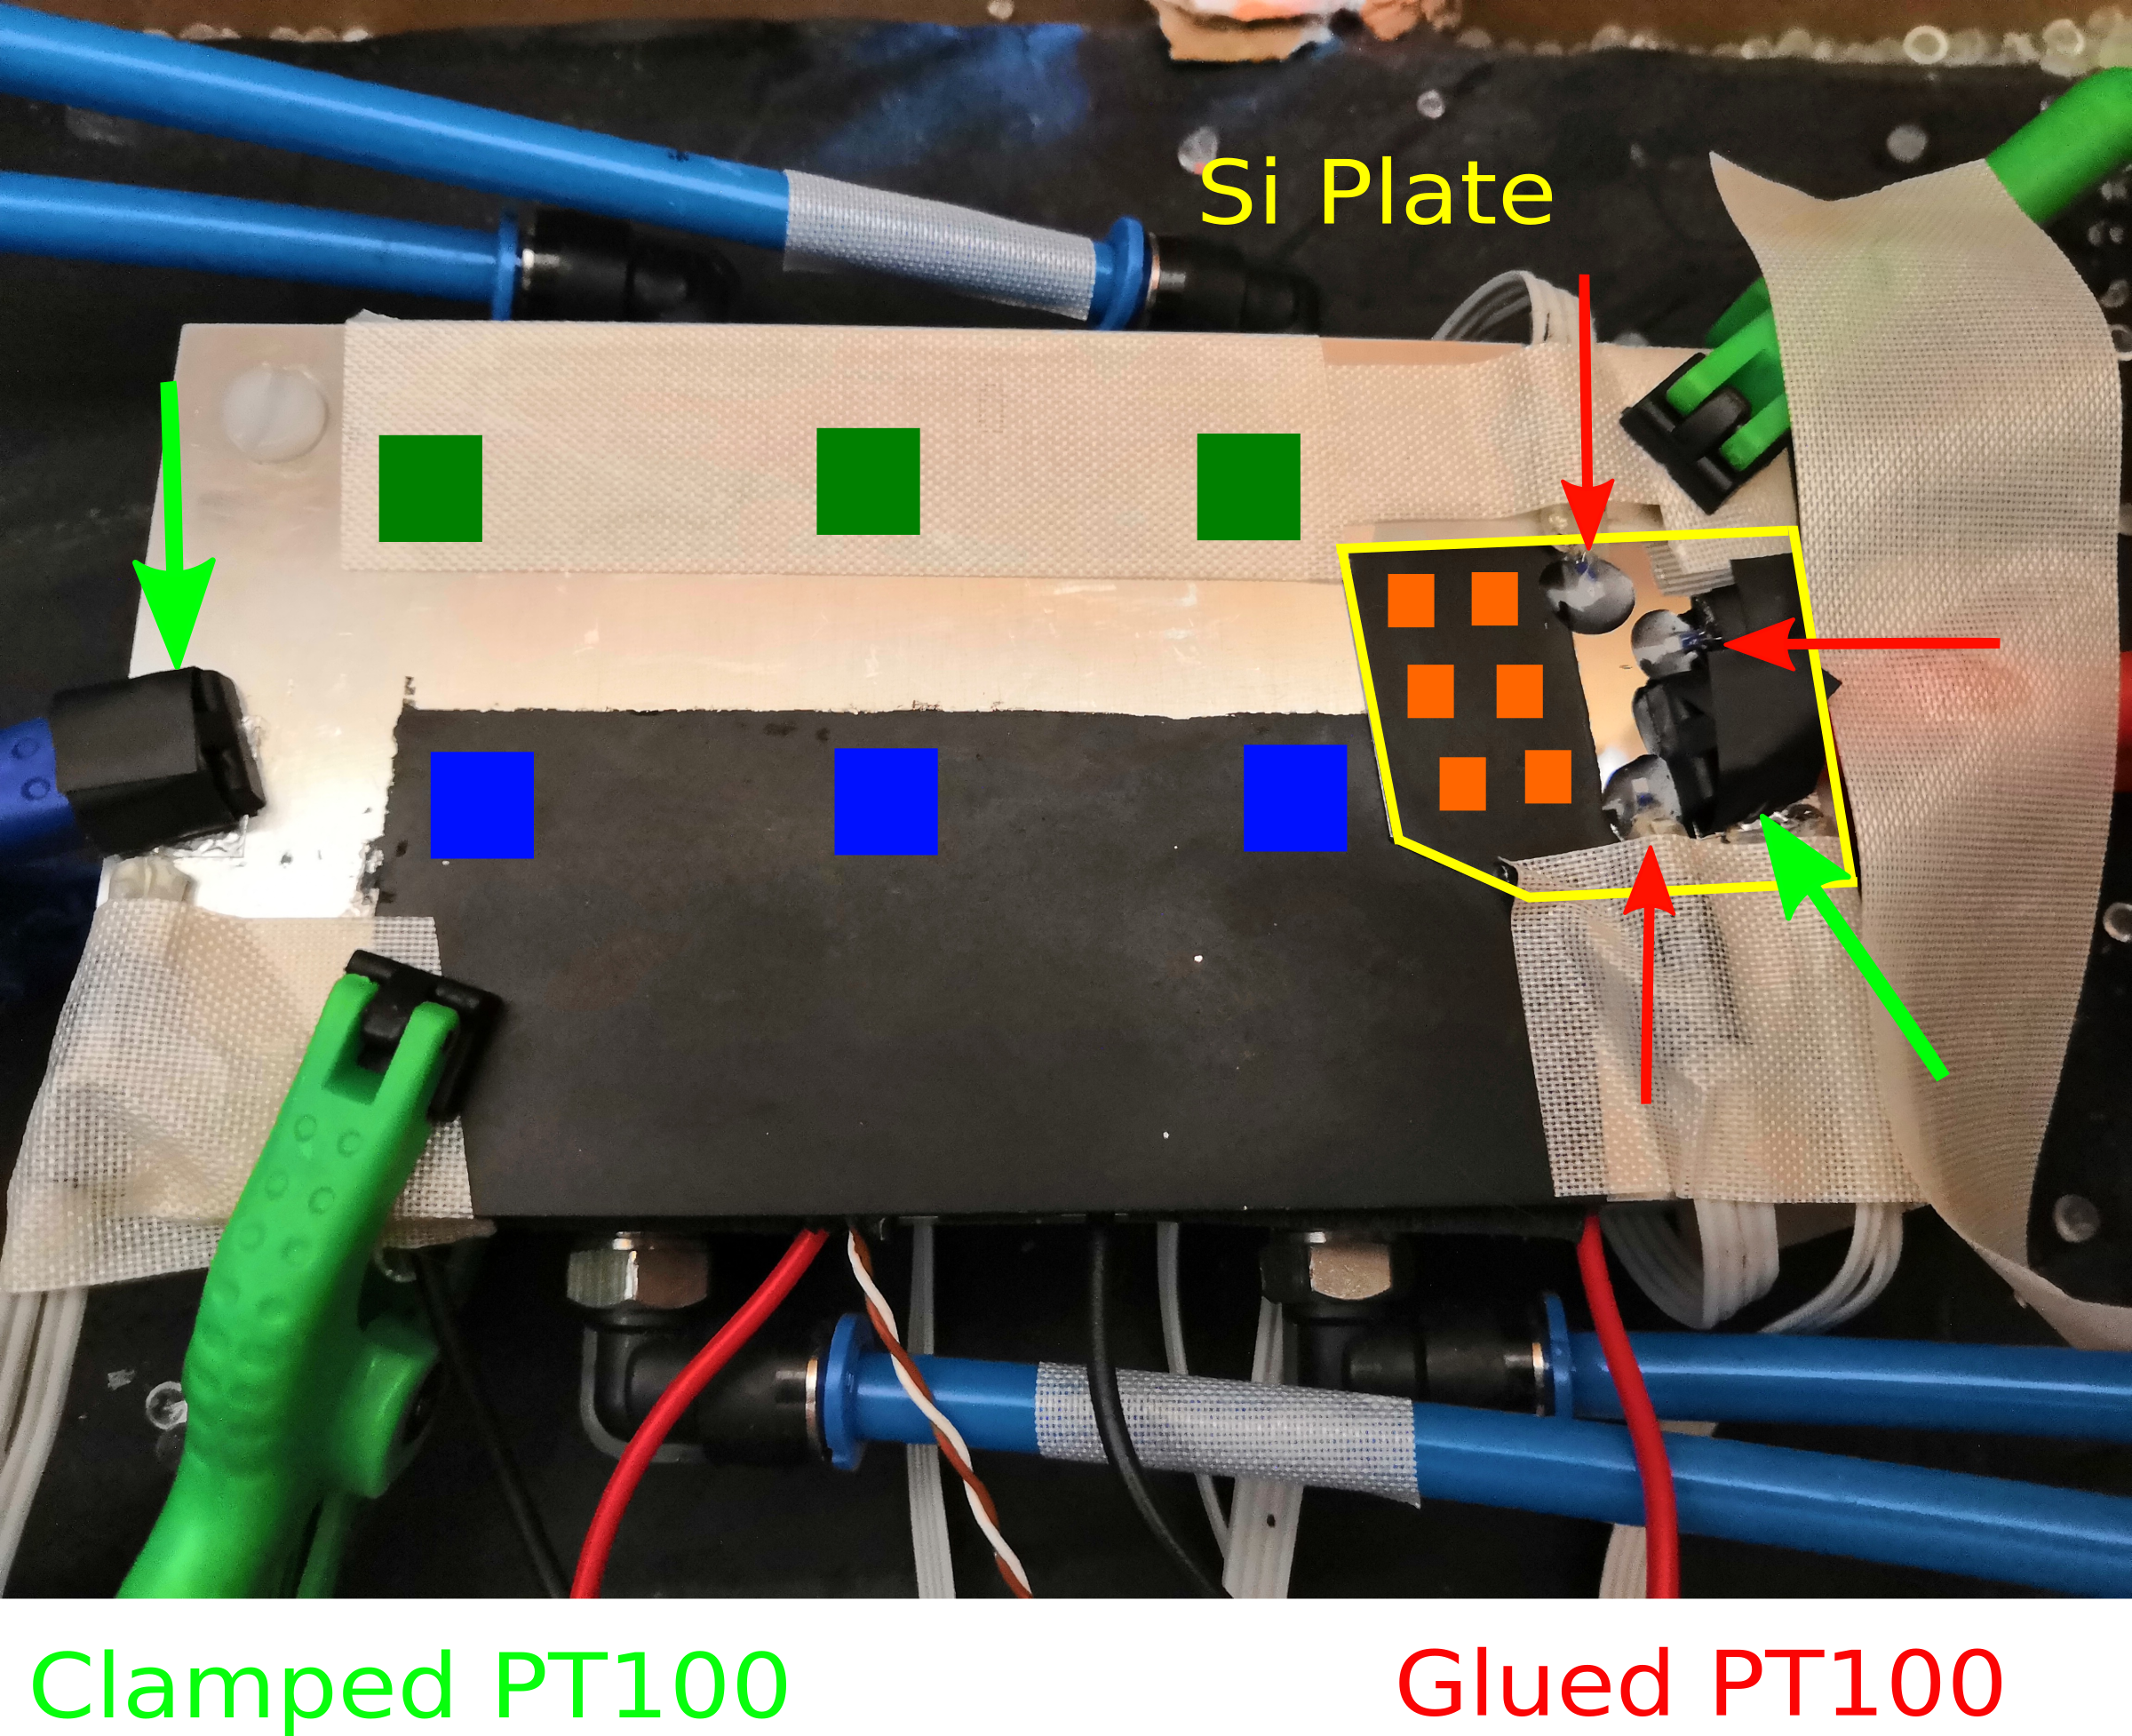
\includegraphics[width=0.6\textwidth]{img/peltierGlued.png}
	\caption{Cold side of the Peltier to test the emissivity of the paint on Si and the reliability of glued pt100s. The Si plate has two parts: one unpainted side with three glued and one clamped pt100, and one painted side with six IR measurement areas. The green and blue squares represent the IR measurement areas on the tape and paint.}
	\label{fig:peltierGlue}
\end{figure}
\subsubsection{Reliability of Glued pt100s}
Figure \ref{fig:glueTemp} compares the temperature measurement of the three glued pt100s and the one clamped pt100s on the Si plate. One of the glued pt100s shows a large deviation whereas the two remaining glued pt100s are rather close to the clamped one. We consider gluing to be a trustworthy measurement overall.
\begin{figure}[h!]
	\centering
	\includegraphics[width=0.7\textwidth]{img/gluing.pdf}
	\caption{Temperatures as measured by the three glued and the one clamped pt100s on the Si.}
	\label{fig:glueTemp}
\end{figure}



\subsubsection{Emissivity of the Paint on Si}
To obtain an emissivity value for the paint on Si, we use again equation \ref{eq:emissivity}, comparing the Si measurement areas with the rightmost tape area. Additionally, we compute again emissivities for the paint on aluminium, comparing each paint area with the closest tape area. Figure \ref{fig:emissivitySi} shows the resulting emissivities. Notably, the values are relatively stable over a broad temperature range and the values for the paint on aluminium are in the range determined in section \ref{sec:emissivityMeasurement}. We expect to have the same emissivity independent of the underlying material. Unfortunately, the emissivities of the paint on Si are higher than this range. We suspect reflections of the clamps, the glue, and the shiny uncoated part of the Si plate to possibly have caused this result. The grouping of the values for the three left and right Si measurement areas supports this argument.
\begin{figure}[h!]
	\centering
	\includegraphics[width=0.7\textwidth]{img/emissivitySi.pdf}
	\caption{Emissivity values for the paint on the Peltier (aluminium) and paint on the Si plate.}
	\label{fig:emissivitySi}
\end{figure}

\subsection{Spraying the Petal}
Intuitively, one would spray the paint onto the petal by laying it on a horizontal surface and spraying from above. This would lead the paint to distribute evenly due to gravitational forces and give a sleek layer of paint. However, number one priority in the spraying process is preserving the wirebonds and the electronics in general. Having a big amount of liquid paint on the petal seems to be too risky which is why we choose to apply the paint from a distance while the petal is in a horizontal position. In figure \ref{fig:petalPreAndPost}, we see the petal before and after the spraying procedure. Figure \ref{fig:petalCloseUp} illustrates the downside of the technique describe above: The paint layer is quite rough and sandy. This does not interfere with the IR measurements given that we cannot observe any Narcissus effect\footnote{Seeing the reflection of the heat emitted by the IR camera in the thermogram when looking at the surface perpendicularly is called Narcissus effect.}.
\begin{figure}[h!]
	\centering
	\begin{subfigure}{\textwidth}
		\includegraphics[width=\textwidth]{img/petal.jpg}
		\caption{Before}
		\label{}
	\end{subfigure} \hfill
	\begin{subfigure}{\textwidth}
		\includegraphics[angle=180, width=\textwidth]{img/entire.jpg}
		\caption{After}
		\label{}
	\end{subfigure}
	\caption{Petal before and after applying the paint.}
	\label{fig:petalPreAndPost}
\end{figure}
\begin{figure}[h!]
	\centering
	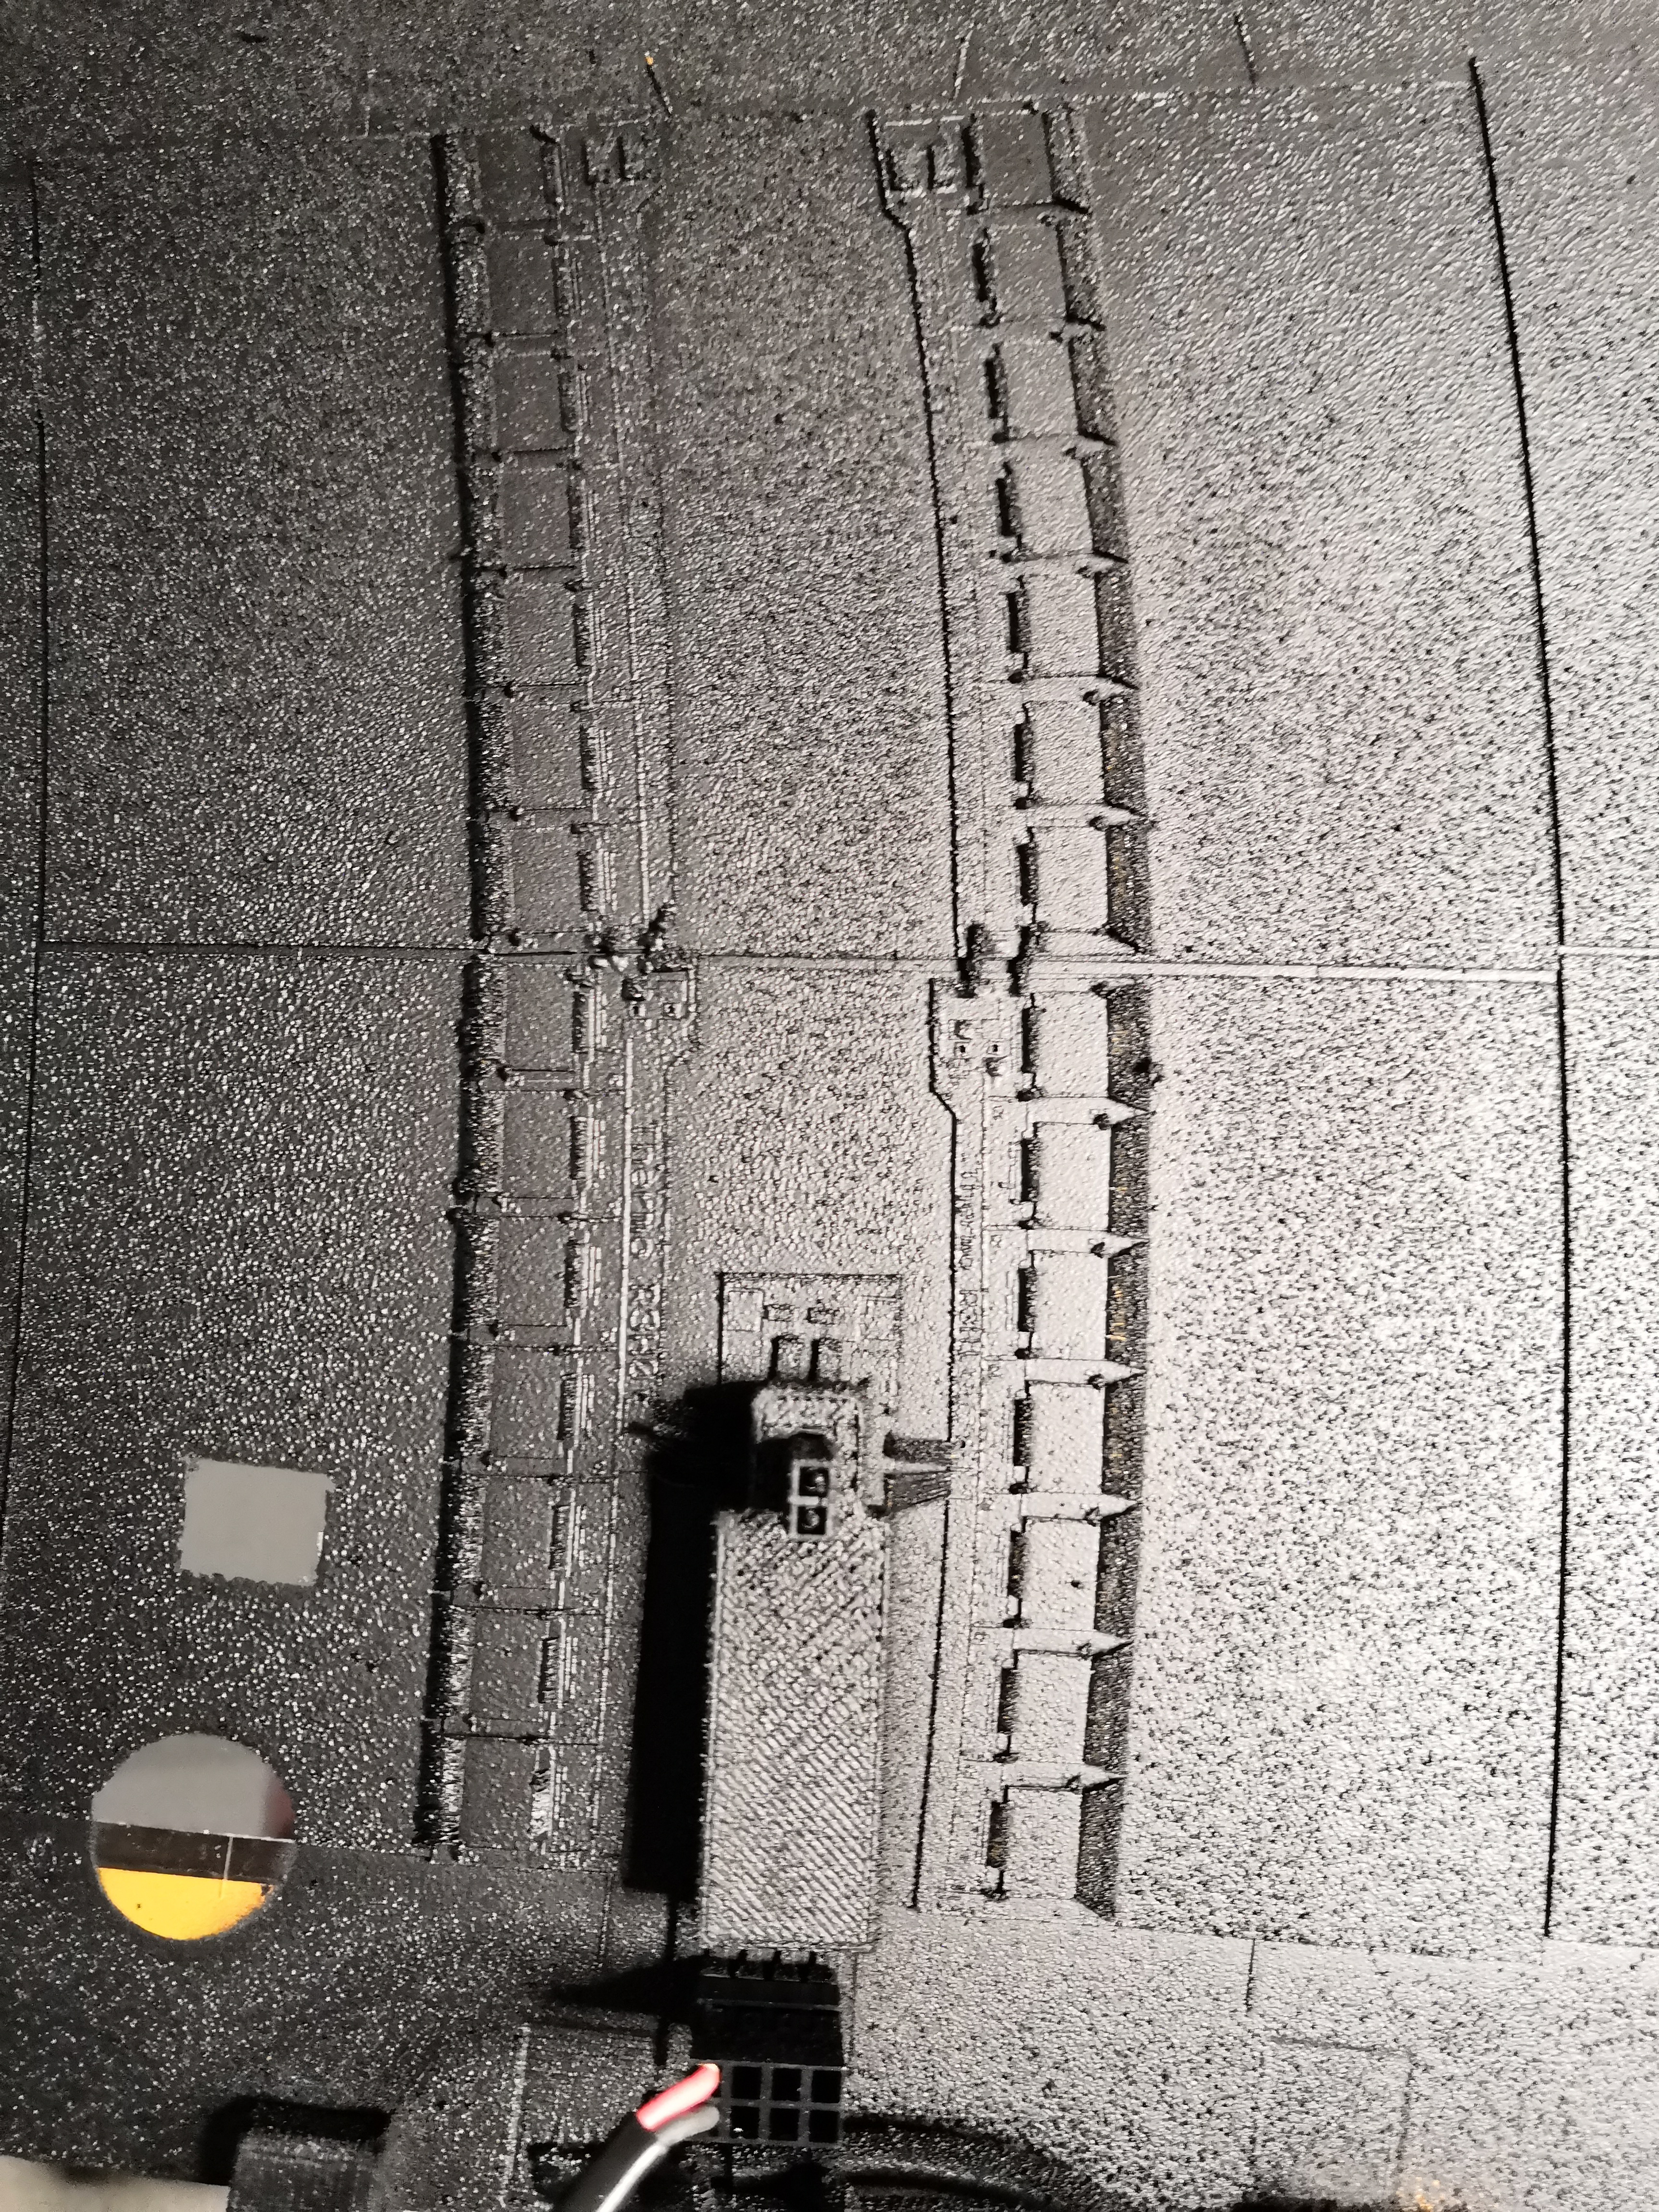
\includegraphics[angle=90, width=0.7\textwidth]{img/R3.jpg}
	\caption{Close up view of the paint structure.}
	\label{fig:petalCloseUp}
\end{figure}

\subsection{First Results}